%% LaTeX-Beamer template for KIT design
%% by Erik Burger, Christian Hammer
%% title picture by Klaus Krogmann
%%
%% version 2.1
%%
%% mostly compatible to KIT corporate design v2.0
%% http://intranet.kit.edu/gestaltungsrichtlinien.php
%%
%% Problems, bugs and comments to
%% burger@kit.edu

\documentclass[18pt]{beamer}

%% SLIDE FORMAT

% use 'beamerthemekit' for standard 4:3 ratio
% for widescreen slides (16:9), use 'beamerthemekitwide'
 
\usepackage{templates/beamerthemekit}
%\usepackage{templates/beamerthemekitwide}

%% TITLE PICTURE

% if a custom picture is to be used on the title page, copy it into the 'logos'
% directory, in the line below, replace 'mypicture' with the 
% filename (without extension) and uncomment the following line
% (picture proportions: 63 : 20 for standard, 169 : 40 for wide
% *.eps format if you use latex+dvips+ps2pdf, 
% *.jpg/*.png/*.pdf if you use pdflatex)

\titleimage{result2017}

%% TITLE LOGO

% for a custom logo on the front page, copy your file into the 'logos'
% directory, insert the filename in the line below and uncomment it

%\titlelogo{mylogo}

% (*.eps format if you use latex+dvips+ps2pdf,
% *.jpg/*.png/*.pdf if you use pdflatex)

%% TikZ INTEGRATION

% use these packages for PCM symbols and UML classes
% \usepackage{templates/tikzkit}
% \usepackage{templates/tikzuml}
\usepackage[utf8]{inputenc}
\usepackage{csquotes}

\usepackage{xcolor}

% define new colors
\definecolor{sql}{HTML}{7F00FF}

% dfeine my own commands
\newcommand{\sql}[1]{%
\texttt{\color{sql}#1}
}


% the presentation starts here

\title[PostgreSQL / PostGIS]{Einführung in (Geo-) Datenbanken:\\ PostgreSQL \& SQL Sprache}
\subtitle{Datenmanagement WS 16/17}
\author{Mirko Mälicke}

\institute{Institut für Wasser und Gewässerentwicklung - Abteilung Hydrologie}

% Bibliography

\usepackage[citestyle=authoryear,bibstyle=numeric,hyperref,backend=biber]{biblatex}
\addbibresource{example.bib}
\bibhang1em

\begin{document}

% change the following line to "ngerman" for German style date and logos
%\selectlanguage{english}
\selectlanguage{ngerman}

%title page
\begin{frame}
\titlepage
\end{frame}

%table of contents
\begin{frame}{Gliederung}
\tableofcontents
\end{frame}

%--------------------------------------------------------
% Einführung
%--------------------------------------------------------
\section{Einführung}

\begin{frame}{Gliederung}
\tableofcontents[currentsection]
\end{frame}\begin{frame}{Über mich}
\begin{itemize}
\item Doktorand am KIT 
\item wissenschaftlicher Mitarbeiter am Felis
\item Schwerpunkt (Geo)Datenmanagement von Umweltdaten
\item räumliche Daten
\item Entwicklung (Python, C++, R, Java, Javascript, SQL)
\item Webentwicklung
\end{itemize}
\end{frame}

\begin{frame}{PostgreSQL Veröffentlichungen}
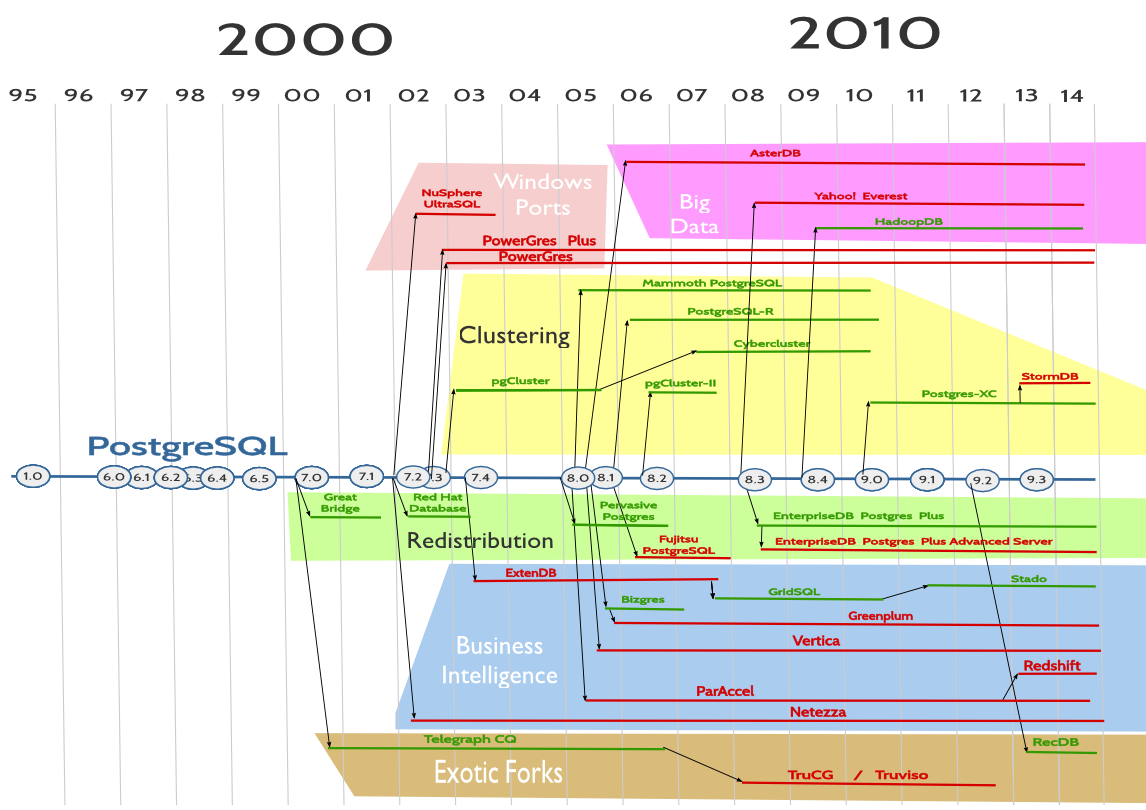
\includegraphics[width=.88\textwidth]{images/TimelinePostgresql}
\end{frame}

\begin{frame}{RDBMS}
\begin{itemize}
\item \textbf{R}elationales \textbf{D}aten\textbf{b}ank \textbf{M}anagement \textbf{S}ystem
\item Ein relationales Datenbankmodell beruht auf der Grundordnung von Daten in Tabellen (=Relationen).
\item Das RDBMS übernimmt die Kommunikation mit der eigentlichen Datenbank. 
\item Die Kommunikationssprache ist \textbf{SQL}.
\item SQL ist eine standardisierte Sprache und damit theoretisch vom RDBMS unabhängig.
\end{itemize}
\end{frame}

\begin{frame}{RDBMS}
\begin{table}
\begin{tabular}{p{.25\textwidth}p{.70\textwidth}}
\textbf{Datensatz} & (=Tupel) ist eine Zeile in einer Tabelle; Duplikate sind nicht zulässig.\\
\textbf{Attribute} & sind Eigenschaften, die einen Datensatz beschreiben, also Spalten in einer Datentabelle. Attribute müssen immer einen Datentyp haben.\\
\textbf{Primärschlüssel} & ist ein (oder mehrere) Attribut das für jedes Tupel eindeutig ist und ihn identifizieren kann. \\
\textbf{Fremdschlüssel} & sind Attribute, die auf den Primärschlüssel anderer Relationen verweisen. \\
\textbf{Kardinalität} & vereinfacht: Beschreibt die Art und Anzahl der zulässigen Verknüpfungen eines (oder mehrerer) Fremdschlüssel.\\
\end{tabular}
\end{table}
\end{frame}

\begin{frame}{Überblick verschiedener RDBMS}
\begin{columns}
\column[c]{.2\textwidth}
	
\includegraphics[width=0.99\textwidth]{images/mysql} 
\column[c]{.8\textwidth}
  \begin{itemize}
  \item Meist genutzte System auf Webservern
  \item seit 2008 kommerzielles System (gibt aber openSource Ableger)
  \end{itemize}
\end{columns}\medskip\par

\begin{columns}
\column[c]{.2\textwidth}
	
\includegraphics[width=0.99\textwidth]{images/sqlite} 
\column[c]{.8\textwidth}
  \begin{itemize}
  \item Keine Server-Anwendung, wird nur in einer Datei abgespeichert
  \item Es gibt für jede Programmiersprache einen Treiber
  \end{itemize}
\end{columns}\medskip\par

\begin{columns}
\column[c]{.2\textwidth}
	
\includegraphics[width=0.99\textwidth]{images/sqlserver} 
\column[c]{.8\textwidth}
  \begin{itemize}
  \item Kommerzielles System von Microsoft 
  \item Zielgruppe sind mittelständische und Großunternehmen
  \item Sehr weit verbreitet
  \end{itemize}
\end{columns}
\end{frame}

\begin{frame}{Überblick verschiedener RDBMS}
\begin{columns}
\column[c]{.2\textwidth}
	
\includegraphics[width=0.99\textwidth]{images/oracle} 
\column[c]{.8\textwidth}
  \begin{itemize}
  \item Am häufigsten eingesetzte RDBMS
  \item gibt auch einen nicht-relationalen Anteil
  \item mit Integriertem Java-Compiler
  \end{itemize}
\end{columns}\medskip\par

\begin{columns}
\column[c]{.2\textwidth}
	
\includegraphics[width=0.99\textwidth]{images/postgres} 
\column[c]{.8\textwidth}
  \begin{itemize}
  \item 100\% open Source; hier weiteste Verbreitung
  \item Sehr viele Erweiterungen, z.B. PostGIS
  \item (quasi) Standard für räumliche Datenbanken
  \item Sehr hoher Anpassungsgrad; dafür jedoch spezifisches Fachwissen nötig
  \end{itemize}
\end{columns}

\end{frame}



%--------------------------------------------------------
% PostgreSQL / PostGIS
%--------------------------------------------------------
\section{PostgreSQL}

\begin{frame}{Gliederung}
\tableofcontents[currentsection]
\end{frame}

\begin{frame}{PostgreSQL}

\begin{columns}
\column[c]{.3\textwidth}
	
\includegraphics[width=0.99\textwidth]{images/postgres} 

\column[c]{.7\textwidth}
	\begin{itemize}
	\item Server-Anwendung, daher Installation eines Postgres Servers erforderlich
    \item Für Windows gibt es kompilierte Installer
    \item Für Linux typischerweise in allen Paketquellen:\\ \texttt{\footnotesize postgres-9.X postgres-9.X-client postgres-server-all-dev}
    \item Der Client ist i.d.R. eine spezifische Anwendung z.B.:
      \begin{itemize}
      \item \texttt{psql} in der Konsole
      \item \texttt{pgAdminIII} als grafische Anwendung
      \end{itemize}
	\end{itemize}
\end{columns}
\end{frame}

%--------------------------------------------------------
% Normalisierung
%--------------------------------------------------------
\section{Normalisierung}

\begin{frame}{Gliederung}
\tableofcontents[currentsection]
\end{frame}

\begin{frame}{Normalisierung}
\begin{itemize}
\item Alleine die relationalen Vorschriften machen noch keine gute Datenbank
\item Eine Datenbank ist immer nur so hilfreich wie ihre Struktur
\item Folglich ein sinnvolles Datenmodell wichtiger als die Wahl des RDBMS 
\item Eine Datenbank muss neben den eigentlichen Daten auch \textbf{alle} Metadaten enthalten
\item Eine Datenbank muss \textbf{immer} dokumentiert sein
\item Faustregel: Struktur so einfach wie möglich aber komplex wie nötig halten
\end{itemize}
\end{frame}

\begin{frame}{Normalisierung}
Zur Sicherstellung der strukturellen Integrität, soll eine Datenbank immer normalisiert werden.\bigskip\par
Durch \textit{Normalisierung} wird ein relationales Datenmodell soweit in einzelne Relationen aufgeteilt und durch Fremdschlüssel verknüpft, bis keine vermeidbaren Redundanzen mehr in den Attribute auftauchen.\bigskip\par
Die Normalisierung unterscheidet 5 hierarchisch aufeinander aufbauende Normalformen
\end{frame}

\begin{frame}{Normalisierung}
\begin{description}
\item [\textbf{1. Normalform}]Die Wertebereiche der Attribute einer Relation müssen atomar sein.
\item [\textbf{2. Normalform}]Jedes Nicht-Schlüssel Attribut muss voll funktional vom Primärschlüssel abhängen.
\item [\textbf{3. Normalform}]Kein Nicht-Schlüssel Attribut darf transitiv von einem Schlüssel Attribut abhängen
\end{description}
\vspace{0.5cm}
\textit{Diese drei Normalformen werden anhand einer Übung veranschaulicht.}
\end{frame}

%--------------------------------------------------------
% SQL
%--------------------------------------------------------
\section{SQL Sprache}

\subsection{Grundlagen}

\begin{frame}{Gliederung}
\tableofcontents[currentsection, currentsubsection]
\end{frame}

\begin{frame}{Grundlagen SQL}
Das erste Schlüsselwort eines SQL Befehls definiert die \textit{Art} der Anfrage, gefolgt von der Datentabelle oder der Funktion die Ziel des Befehls ist. Ein SQL Befehl wird mit einem Semikolon abgeschlossen (Bei einzelnen Befehlen kann dies weg gelassen werden).
\begin{description}
\item [\sql{SELECT}] Ruft Daten aus einer Datentabelle ab / eine Funktion auf.
\item [\sql{INSERT}] Fügt ein neues Tupel in eine Relation ein.
\item [\sql{UPDATE}] Ändert bestehende Daten.
\item [\sql{DELETE}] Löscht Daten aus einer Relation.
\end{description}
\textit{\footnotesize\sql{DELETE} bezieht sich immer nur auf Daten, zum löschen eines Strukturelements wird \sql{DROP} verwendet.}
\end{frame}

\begin{frame}{Beispiele}
\textit{\sql{SELECT} * \sql{FROM} houses}\bigskip\par
\textit{\sql{SELECT} street, number \sql{FROM} houses}\bigskip\par
\textit{\sql{SELECT} * \sql{FROM} houses \sql{WHERE} owner='Freiburg'}\bigskip\par
\end{frame}

\begin{frame}{Beispiele}
\textit{\sql{SELECT} count(*) \sql{FROM} houses \sql{WHERE} owner='Freiburg'}\bigskip\par
\textit{\sql{SELECT DISTINCT} fr\_str\_full\_name \sql{AS} "'Namen"' \sql{FROM} street}\bigskip\par
\textit{\sql{SELECT} 15 / 4}\bigskip\par
\textit{\sql{SELECT} 15::\sql{real} / 4::\sql{real}}
\end{frame}


\subsection{Gruppierung}

\begin{frame}{Gliederung}
\tableofcontents[currentsection, currentsubsection]
\end{frame}

\begin{frame}{Gruppieren}
Eine der größten Stärken einer Datenbank ist ihre Fähigkeit Daten zu gruppieren (aggregieren) und somit noch vor der Transaktion zum Client das Datenaufkommen zu minimieren. Hierfür wird das Schlüsselwort \sql{GROUP BY} \textit{Spalte} verwendet. Nun gruppiert die Datenbank nach der angegebenen Spalte(n).\\
Wichtig ist, dass alle Spalten, nach denen nicht gruppiert wird über eine Funktion zusammenfassbar sind oder nur den selben Wert enthalten.
\end{frame}
\begin{frame}{Gruppieren}
\textit{\sql{SELECT} woche, min(value) \sql{AS} "'Minimum"', max(value) \sql{AS} "'Maximum"' \sql{FROM} data \sql{GROUP BY} woche}\bigskip\par
\end{frame}

\subsection{Nesting}
\begin{frame}{Gliederung}
\tableofcontents[currentsection, currentsubsection]
\end{frame}

\begin{frame}{Nested SELECT}
\begin{itemize}
\item SQL \sql{SELECT} Abfragen können beliebig verschachtelt werden
\item Jede geschlossene Abfrage kann mit \sql{AS} einen Alias bekommen und verhält sich dann wie eine Tabelle
\bigskip\par
\item Syntax: \textit{\sql{SELECT} t.col, t.col2 \sql{FROM} (\sql{SELECT} \ldots \sql{FROM} \ldots) \sql{AS} t}
\end{itemize}
\end{frame}

\subsection{Views}
\begin{frame}{Gliederung}
\tableofcontents[currentsection, currentsubsection]
\end{frame}

\begin{frame}{VIEWs}
\begin{itemize}
\item Ein \sql{VIEW} ist eine dynamische Datenansicht
\item Verhält sich wie eine Tabelle, wird jedoch bei jeder Abfrage neu erstellt
\item \sql{INSERT, UPDATE} und \sql{DELETE} funktionieren bei einem \sql{VIEW} nicht
\bigskip\par
\item Syntax: \textit{\sql{CREATE VIEW} view\_name \sql{AS} \sql{SELECT} \ldots \sql{FROM} \ldots }
\end{itemize}
\end{frame}



%--------------------------------------------------------
% Räumliche Abfrage
%--------------------------------------------------------
\section{Räumliche Abfragen}

\begin{frame}{Gliederung}
\tableofcontents[currentsection]
\end{frame}

\begin{frame}{Grundfunktionen}
\begin{itemize}
\item \texttt{st\_AsEWKT(\textit{geom})} transferiert eine binäre Geometrie in ein WKT
\item \texttt{st\_GeomFromText(\textit{WKT}, \textit{srid})} erzeugt eine binäre Geometrie aus einem WKT
\item \texttt{st\_SetSRID(\textit{geom}, \textit{srid})} verknüpft die Geometrie mit dem angegebenen CRS (Achtung! kein Transform)
\item \texttt{st\_Transform(\textit{geom}, \textit{srid})} transformiert die Geometrie in das angegebene CRS
\item \texttt{st\_Transform(\textit{geom}, \textit{from\_srid}, \textit{to\_srid})} transformiert die Geometrie vom CRS from\_srid in das CRS to\_srid
\end{itemize}\medskip\par
\textit{Was ist der Unterschied zwischen st\_setsrid und st\_transform?}
\end{frame}

\begin{frame}{Räumliche Relation}
\begin{itemize}
\item \texttt{st\_Within(\textit{g1}, \textit{g2})} gibt \sql{TRUE} zurück wenn g2 komplett innerhalb g1 liegt
\item \texttt{st\_Intersects(\textit{g1}, \textit{g2})} gibt \sql{TRUE} zurück wenn g1 und g2 gemeinsame Punkte haben, die nicht zum Rand gehören.
\item \texttt{st\_Disjoint(\textit{g1}, \textit{g2})} gibt \sql{TRUE} zurück wenn g1 und g2 keine gemeinsamen Punkte besitzen
\item \texttt{st\_Touches(\textit{g1}, \textit{g2})} gibt \sql{TRUE} wenn g1 und g2 gemeinsame Punkte haben, die ausschließlich zum Rand gehören
\end{itemize}
\end{frame}

\begin{frame}{GIS}
\begin{itemize}
\item \texttt{st\_Distance(\textit{g1}, \textit{g2})} Berechnet den Abstand der Geometrien g1 und g2
liegt
\item \texttt{st\_Buffer(\textit{g1}, \textit{radius})} Berechnet einen Puffer mit Abstand \textit{radius} um g1
\item \texttt{st\_Intersection(\textit{g1}, \textit{g2})} Berechnet die Schnittmenge aus g1 und g2
\item \texttt{st\_Union(\textit{g1}, \textit{g2})} Berechnet die Vereinigung aus g1 und g2
\end{itemize}
\end{frame}


%--------------------------------------------------------
% PostGIS und QGis
%--------------------------------------------------------
\section{PostGIS \& QGis}

\begin{frame}{Gliederung}
\tableofcontents[currentsection]
\end{frame}



%\begin{frame}{Example slide B}
%\begin{block}{Block 1}
%\begin{itemize}
%\item Bullet point 1
%\pause
%\item Bullet point 2
%\item \dots
%\end{itemize}
%\end{block}
%\end{frame}

%\begin{frame}{Example slide C}
%\begin{exampleblock}{Example 1}
%\begin{itemize}
%\item Bullet point 1
%\pause
%\item Bullet point 2
%\item \dots
%\end{itemize}
%\end{exampleblock}
%\end{frame}

%\begin{frame}{Example slide D}
%\begin{alertblock}{Alert 1}
%\begin{itemize}
%\item Bullet point 1
%\pause
%\item Bullet point 2
%\item \dots
%\end{itemize}
%\end{alertblock}
%\end{frame}

\appendix
\beginbackup

%\begin{frame}[allowframebreaks]{References}
%\printbibliography
%\end{frame}

\backupend

\end{document}
